
\chapter{Libraries}

\begin{definitionblock}
    A library is a collection of pre-written code or routines that can be reused by computer programs.
    These libraries typically contain functions, variables, classes, and procedures that perform
    common tasks, allowing developers to save time and effort by leveraging existing code rather than
    writing everything from scratch.
\end{definitionblock}

Why are useful? 
\begin{itemize}
    \item \textbf{Text Reusability}: Libraries provide a set of functionalities that can be used across multiple
    projects, reducing the need to write the same code over and over again.
    \item \textbf{Modularity}: Libraries promote modular programming by encapsulating specific functionalities
    into separate modules or components.
    \item \textbf{Abstraction}: Libraries abstract the underlying implementation details, allowing developers to
    use high-level interfaces without needing to understand the inner workings of the functions
    provided by the library.
    \item \textbf{Collaboration}: Communities of developers can share and collaborate on libraries,
    accelerating the development process. Many programming languages have centralized
    repositories or package managers to facilitate the distribution and installation of libraries.
    \item \textbf{Efficiency}: Libraries are often optimized and well-tested, providing efficient and reliable
    solutions for common programming tasks.
\end{itemize}

Libraries are composed by:
\begin{itemize}
    \item \textbf{Header Files}: Header files contain declarations of functions, variables, and classes that are
    defined in the library. They provide the necessary information for the compiler to link the
    library with the program.
    \item \textbf{Source Files}: Source files contain the actual implementation of the functions, variables, and
    classes declared in the header files. They are compiled into object files that are linked together
    to create the final executable. They can be either static or shared. 
\end{itemize}

\begin{observationblock}[Header-only libraries]
An exception are the libraries that contain only header files, which are known as header-only libraries.
\end{observationblock}

Header files are only used in the development phase. In production, only \textbf{library files} are
needed. Precompiled executables that just use shared libraries do not need header files to work. This is
why certain software packages are divided into standard and development versions; only the latter
contains the full set of header files.

\begin{figure}[H]
    \centering
    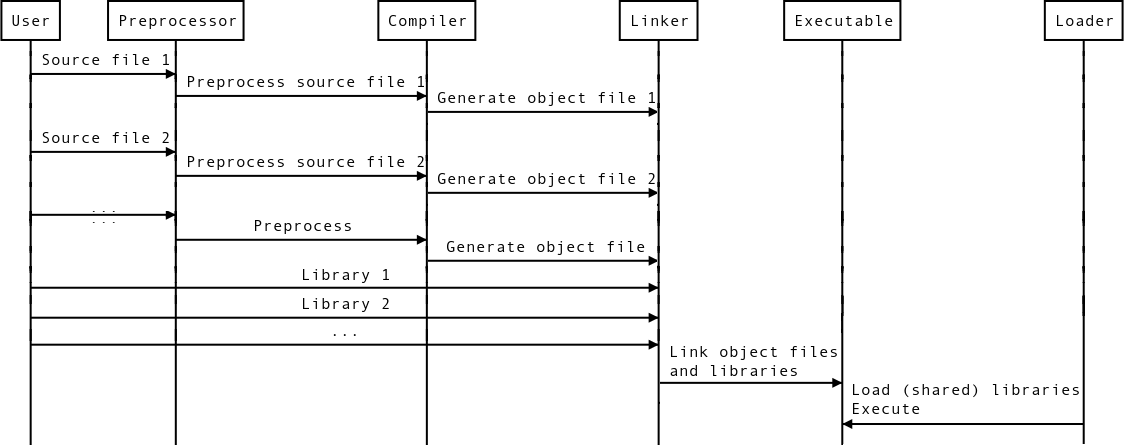
\includegraphics[width=\textwidth]{assets/build_process.png}
    \caption{Build Process}
\end{figure}

Another distinction has to be made:
\begin{itemize}
    \item \textbf{Static Libraries}: Static libraries are linked directly into the executable at compile time. Denoted with \texttt{.a} or \texttt{.lib} extension. When you build a program using a static library, a copy of the library's code is
    included in the final executable. This means that the resulting executable is independent of
    the original library file; it contains all the necessary code to run without relying on external
    library files.
    \item \textbf{Shared Libraries}: Shared libraries are loaded at runtime when the program is executed. Denoted with \texttt{.so} or \texttt{.dll} extension. When you build a program using a shared library, the library file is not included in the
    executable. Instead, the program references the shared library file, which is loaded into memory
    when the program is run. This allows multiple programs to share the same library file, reducing
    the overall memory footprint.
\end{itemize}

\section{The build process}

The preprocessing and compilation steps
\begin{codeblock}[language=bash]
    g++ -Imylib/include -c main.cpp -o main.o
\end{codeblock}
produce the main.o executable, it contains 
\begin{codeblock}[language=bash]
$ nm -C main.o
0000000000000000 T main
                 U my_fun
\end{codeblock}

The \texttt{T} in the second column indicates that the function \texttt{main\(\)} is actually defined (resolved) by
the library. While \texttt{myfun\(\)} is referenced but undefined. So, to produce a working executable, you
have to specify to the linker another library or object file where it is defined.

\subsection*{Case 1: You can access \textit{myfun\(\)}}

\begin{itemize}
    \item compile the object file implementing the function
    \begin{codeblock}
        g++ -c mylib.cpp 
    \end{codeblock}
    \item link the application against that object file 
    \begin{codeblock}
    g++ main.o mylib/mylib.o -o main 
    \end{codeblock}
    \item now both \texttt{main} and \texttt{myfun} are resolved 
    \begin{codeblock}
    $ nm -C main
    0000000000000000 T main
    0000000000000010 T my_fun
    \end{codeblock}
\end{itemize}

\subsection*{Case 2: The reality}

In reality there are problems with this approach:
\begin{itemize}
    \item Compilation takes time! 
    \item Recompilation has to be done every time the library changes
    \item Actual implementation of the library is not available most of the times 
    \item Dependency Hell 
\end{itemize}

You can link in two ways:
\begin{codeblock}[language=bash]
    g++ main.o /path/to/mylib/libmylib.a -o main  # using library full path
\end{codeblock}
\begin{codeblock}[language=bash]
    g++ main.o -L/path/to/mylib -lmylib -o main  # using -L and -l flags
\end{codeblock}

\begin{warningblock}
    The order of the arguments is important! The linker processes the arguments from left to right, so
    the libraries should be specified after the object files that reference them.
\end{warningblock}


\section{Static Libraries}
Static libraries are the oldest and most basic way of integrating third-party code. They are basically
a collection of object files stored in a single archive.
At the linking stage of the compilation processes, the symbols that are still unresolved are
searched into the other object files indicated to the linker and in the indicated libraries, and
eventually the corresponding code is inserted in the executable.

Libraries result themselves from preprocessing and compiling their corresponding source codes. 

\begin{codeblock}[language=bash]
    g++ -c mylib.cpp
    ar rcs libmylib.a mylib.o
\end{codeblock}

\begin{definitionblock}
A static library is just an archive of source codes.
\end{definitionblock}

\begin{figure}[H]
    \centering
    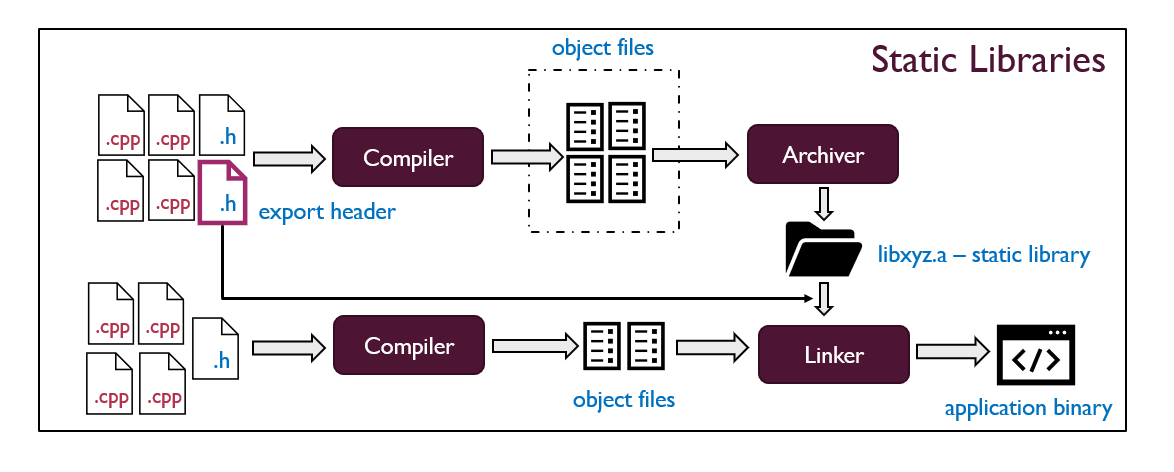
\includegraphics[width=\textwidth]{assets/static_lib.png}
    \caption{Static Library}
\end{figure}

\subsection*{Creating A Static Library}

\begin{figure}[H]
    \centering
    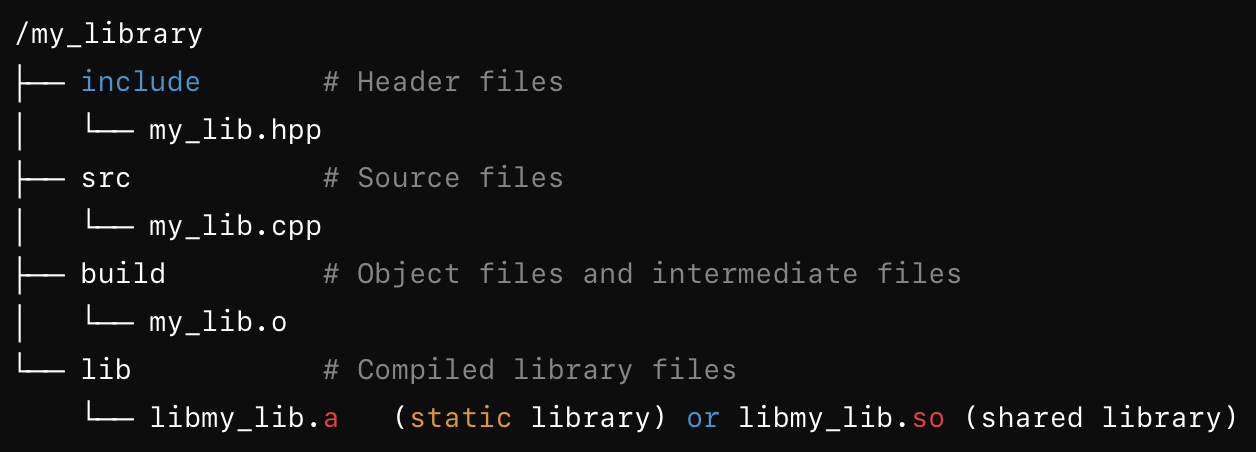
\includegraphics[width=\textwidth]{assets/library_directory.png}
    \caption{Directory Structure}
\end{figure}

First create a folder (/my\_library) with sub-folders /include (for header\_files.hpp), /src (for source\_files.cpp), /build (for compiled.o files) and /lib (for compiled\_library\_files.a).

Now insert declarations in header\_files.hpp and definitions in source\_files.cpp:

\begin{codeblock}[language=C++]
    // chrislib.hpp
    #pragma once
    
    namespace chrislib {
    
        void hello_world();  // Function declaration
    
    }
\end{codeblock}

\begin{codeblock}[language=C++]
    // chrislib.cpp
    #include "/path_to_library/include/chrislib.hpp"
    #include <iostream>
    
    namespace chrislib {
    
        void hello_world() {
            std::cout << "Hello from my private library!" << std::endl;
        }
    
    }
\end{codeblock}


And then with terminal compile the source files:

\begin{codeblock}[language=bash]
g++ -c src/chrislib.cpp -o build/chrislib.o   ## compilation
ar rcs lib/libmy_lib.a build/my_lib.o   ## library files
\end{codeblock}

Now you have the executables needed to use the library. It is time to create the project directory.


\subsection*{Using A Static Library}

\begin{figure}[H]
    \centering
    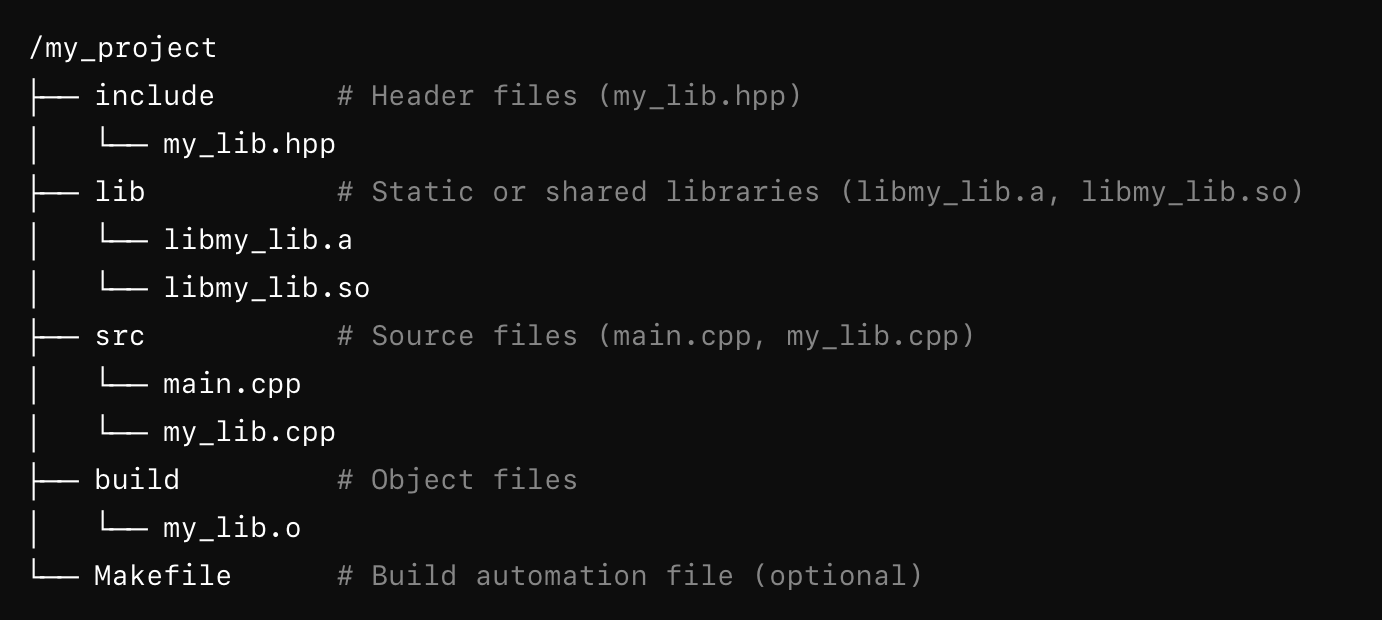
\includegraphics[width=\textwidth]{assets/static_proj_dir.png}
    \caption{Project Directory}
\end{figure}



\begin{codeblock}[language=bash]
    cp -r ~/path_to_library/include ~/project   ## copying the entire include folder
    cp -r ~/path_to_library/lib ~/project   ## copying the entire lib folder
\end{codeblock}

Create now your main.cpp file and compile it.

\begin{codeblock}[language=C++]
    // main.cpp
    #include <iostream>
    #include "/path_to_project/include/chrislib.hpp"
    
    int main() {
        std::cout << "Calling function from my private library!" << std::endl;
        chrislib::hello_world();  // Function from the static library
        return 0;
    }
\end{codeblock}

\vspace{1cm}
\begin{codeblock}[language=bash]
    g++ src/main.cpp -I./include -L./lib -lchrislib -o ./build/test_1   ## -I for headers, -L for library files (executables)
\end{codeblock}

Now just run the file (test\_1):
\begin{codeblock}[language=bash]
    christianfaccio@Christians-MacBook-Air build % ./test_1
    Calling function from my private library!
    Hello from my private library!
\end{codeblock}


\subsection*{Key Flags:}
\begin{itemize}
    \item \textbf{-I} \textit{(Include Directory)}: Specifies the directory to search for header files. 
    \[
    \texttt{-I /path/to/include}
    \]
    
    \item \textbf{-L} \textit{(Library Directory)}: Specifies the directory to search for static libraries.
    \[
    \texttt{-L /path/to/lib}
    \]

    \item \textbf{-l} \textit{(Link Library)}: Links the static library (without the \texttt{lib} prefix and file extension).
    \[
    \texttt{-lchrislib}
    \]

    \item \textbf{-o} \textit{(Output File)}: Specifies the output executable name.
    \[
    \texttt{-o my\_program}
    \]

    \item \textbf{-std=c++17} \textit{(C++ Standard)}: Specifies the C++ version to use (e.g., C++17).
    \[
    \texttt{-std=c++17}
    \]

    \item \textbf{-Wall} \textit{(All Warnings)}: Enables all compiler warnings.
    \[
    \texttt{-Wall}
    \]

    \item \textbf{-g} \textit{(Debug Information)}: Includes debugging information in the compiled binary.
    \[
    \texttt{-g}
    \]

    \item \textbf{-r} \textit{(Relocatable Object File)}: Tells the linker to generate an object file that is relocatable (not yet fully linked). 
    \[
    \texttt{-r}
    \]
\end{itemize}



\section{Shared Libraries}

Here:
\begin{itemize}
    \item The \textbf{linker} ensures that symbols that are still unresolved are provided by the library. 
    \item The corresponding code is not inserted, and the symbols remain unresolved.
    \item Instead, a reference to the library is stored in the executable for later use by the \textbf{loader}.
\end{itemize}

\begin{warningblock}
    Linker and loader are two different programs!
\end{warningblock}

\begin{figure}[H]
    \centering
    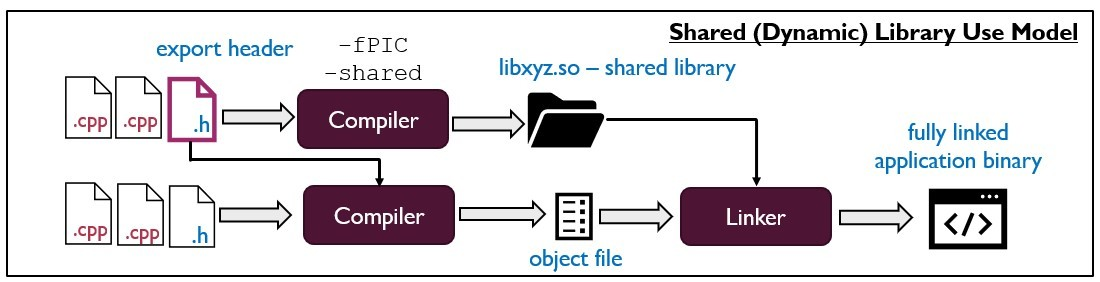
\includegraphics[width=\textwidth]{assets/dynamic_lib.jpeg}
    \caption{Shared Library}
\end{figure}

\subsection*{Creating A Shared Library}

As before, create the header\_files.hpp and source\_files.cpp (I will use the same as before), putting them in a directory with the same structure as before. 
\begin{codeblock}[language=bash]
g++ -fPIC -shared -Iinclude src/chrislib.cpp -o lib/libchrislib.so  ## you can even create the executable .o but it is an intermediary step
\end{codeblock}

\begin{figure}[H]
    \centering
    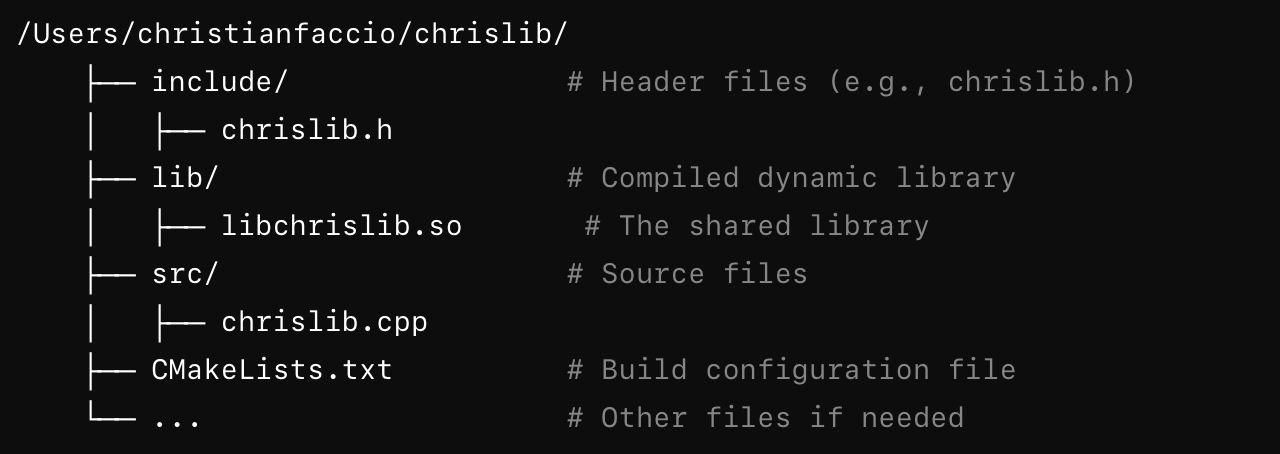
\includegraphics[width=\textwidth]{assets/dynamic_lib_dir.png}
    \caption{Shared Library}
\end{figure}

\subsection*{Using A Shared Library}


Go to the project directory, then
\begin{codeblock}[language=bash]
g++ -I../chrislib/include -L../chrislib/lib -lchrislib src/main.cpp -o build/my_program  
\end{codeblock}
\begin{codeblock}[language=bash]
export LD_LIBRARY_PATH=../chrislib/lib:$LD_LIBRARY_PATH
\end{codeblock}
\begin{codeblock}[language=bash]
christianfaccio@Christians-MacBook-Air project_test % ./build/my_program  ## run the program
Hello from chrislib!
\end{codeblock}

\begin{figure}
    \centering
    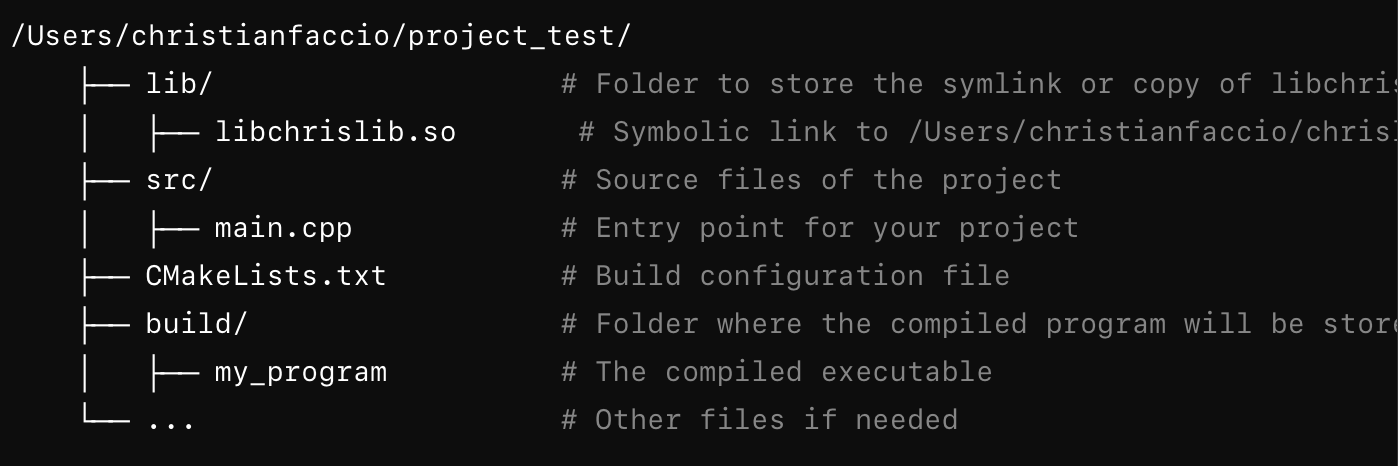
\includegraphics[width=\textwidth]{assets/dynamic_proj_dir.png}
    \caption{Shared Library}
\end{figure}

\subsection*{Key Flags:}
\begin{itemize}
    \item \texttt{-fPIC}: Generate position-independent code (required for shared libraries).
    \item \texttt{-shared}: Create a shared library.
\end{itemize}

\subsection*{Linking and Compilation Flags}


\begin{itemize}
    \item \textbf{-I} \textit{(Include Directory)}: Specifies the directory to search for header files.
    \[
    \texttt{-I /path/to/include}
    \]
    
    \item \textbf{-L} \textit{(Library Directory)}: Specifies the directory to search for shared libraries.
    \[
    \texttt{-L /path/to/lib}
    \]

    \item \textbf{-l} \textit{(Link Library)}: Links the shared library (without the \texttt{lib} prefix and file extension).
    \[
    \texttt{-lchrislib}
    \]

    \item \textbf{-o} \textit{(Output File)}: Specifies the output executable name.
    \[
    \texttt{-o my\_program}
    \]

    \item \textbf{-fPIC} \textit{(Position Independent Code)}: Tells the compiler to generate position-independent code for shared libraries.
    \[
    \texttt{-fPIC}
    \]

    \item \textbf{-shared} \textit{(Create Shared Library)}: Tells the compiler to create a shared library.
    \[
    \texttt{-shared}
    \]

    \item \textbf{-Wl,-rpath} \textit{(Runtime Library Search Path)}: Specifies a runtime path for shared libraries.
    \[
    \texttt{-Wl,-rpath,/path/to/lib}
    \]

    \item \textbf{-std=c++17} \textit{(C++ Standard)}: Specifies the C++ version to use (e.g., C++17).
    \[
    \texttt{-std=c++17}
    \]

    \item \textbf{-Wall} \textit{(All Warnings)}: Enables all compiler warnings.
    \[
    \texttt{-Wall}
    \]

    \item \textbf{-g} \textit{(Debug Information)}: Includes debugging information in the compiled binary.
    \[
    \texttt{-g}
    \]
\end{itemize}

\section{Version Control}

The version is an identifier typically represented by a sequence of numbers, indicating instances
of a library with a common public interface and functionality. 
Naming scheme:
\begin{itemize}
    \item \textbf{Link Name}: Used in the linking stage with the -lmylib option, of the form libmylib.so 
    \item \textbf{soname (shared object name)}: Looked after by the loader, typically formed by the link
    name followed by the major version number, e.g., libmylib.so.3 
    \item \textbf{Real Name}: The actual file storing the library with the full version number, e.g.,
    libmylib.so.3.2.4
\end{itemize}

The ldd command is used (Linux/Mac) to display the shared libraries required by a program or a shared library. It shows the list of dynamic libraries (shared objects) that are linked to an executable or a shared library at runtime.

\begin{codeblock}[language=bash]
/Users/christianfaccio/project_test/lib/libchrislib.so:
\end{codeblock}
\begin{codeblock}[language=bash]
build/libchrislib.so (compatibility version 0.0.0, current version 0.0.0)
/usr/lib/libc++.1.dylib (compatibility version 1.0.0, current version 1800.101.0)
/usr/lib/libSystem.B.dylib (compatibility version 1.0.0, current version 1351.0.0)
\end{codeblock}

If there's a new release, placing the corresponding file in the /lib directory and resetting symbolic links, will make the program use the new release without recompiling (and this is what happens when, for example, you upgrade a package via apt or similar).

When working with different versions of libraries, dependency management becomes important to ensure that the correct versions of libraries are linked and used by your applications. This is especially crucial when there are multiple versions of libraries on your system, as using an incorrect version may lead to runtime errors or unexpected behavior.

\begin{itemize}
    \item \textbf{Compatilbility version}: The version that a shared library guarantees compatibility with. This means that any program or library that links to this version will work as expected with the shared library
    \item \textbf{Current version}: The actual version of the library. It can evolve over time with bug fixes, features, or breaking changes
\end{itemize}

If you're using symbolic links (e.g., libchrislib.so pointing to a specific version like libchrislib.1.so), ls -l will show you where the symlink points.

\begin{codeblock}[language=bash]
ls -l /path/to/libchrislib.so
\end{codeblock}
\begin{codeblock}[language=bash]
lrwxr-xr-x  1 christianfaccio  staff  52 Nov 14 23:32 /Users/christianfaccio/project_test/lib/libchrislib.so -> /Users/christianfaccio/chrislib/build/libchrislib.so
\end{codeblock}



SONAME is a special name associated with shared libraries that helps the system identify which version of the library to load at runtime. It is used to manage compatibility between different versions of the same library. When a library is built and installed, the SONAME is embedded in the file as part of the dynamic linking process. This allows executables that rely on that library to load the correct version during runtime, based on the version specified in the SONAME. 

For example, if you have a libchrislib.so.1 library (version 1) and you update it to libchrislib.so.2 (version 2), the SONAME might still reference libchrislib.so.1, ensuring older programs using version 1 of the library work as expected.

When creating a shared library, you typically specify the SONAME using the -Wl,-soname flag during compilation and linking. For example:

\begin{codeblock}[language=bash]
gcc -shared -o libchrislib.so.1.2.3 -Wl,-soname,libchrislib.so.1 chrislib.o
\end{codeblock}

This will ensure that the SONAME libchrislib.so.1 is embedded in the library file, and any application that links against libchrislib.so.1 will use this specific version or a compatible version.

\subsection*{Loading Phase}

Linking and Loading phases are different. The loader has a different search strategy with respect to the linker. It looks in /lib , /usr/lib ,
and in all the directories contained in /etc/ld.conf or in files with the extension conf contained
in the /etc/ld.conf.d/ directory.








